\documentclass[10pt,journal,compsoc]{IEEEtran}
% Target venue: IEEE Transactions on Pattern Analysis and Machine Intelligence
\usepackage{amsmath,amssymb,amsthm,mathtools}
\usepackage{booktabs}
\usepackage{graphicx}
\usepackage[noadjust]{cite}
\usepackage{url}
\usepackage{algorithm}
\usepackage{algpseudocode}

\newtheorem{theorem}{Theorem}
\newtheorem{lemma}{Lemma}
\newtheorem{proposition}{Proposition}
\newtheorem{corollary}{Corollary}
\newtheorem{assumption}{Assumption}
\newtheorem{remark}{Remark}
\newcommand{\R}{\mathbb{R}}
\newcommand{\E}{\mathbb{E}}
\newcommand{\dd}{\mathrm{d}}
\newcommand{\TV}{\mathrm{TV}}
\graphicspath{{figs/}}

\begin{document}

\title{Fast, Efficient, and Exact MCMC:\\ Learned Residual Transport Atlases with\\ Zero-Gradient Production Sampling}

\author{Bhum~Soonjun%
\thanks{Draft manuscript. Code, all benchmark artifacts, and reproduction
scripts accompany the submission.}}

\IEEEtitleabstractindextext{%
\begin{abstract}
We introduce a Markov chain Monte Carlo sampler that is simultaneously
\emph{fast} (native production kernel at $0.3$--$47\,\mu$s per draw),
\emph{efficient} (up to three orders of magnitude fewer oracle evaluations per
effective sample than the No-U-Turn Sampler), and \emph{exact} (the invariant
law is the target posterior for any fixed surrogate, verified by
simulation-based calibration). The method separates inference into a finite
warm-up that \emph{learns geometry} and a frozen production phase that
\emph{never evaluates the target gradient} and evaluates the target density
exactly once per transition. Warm-up constructs a \emph{transport atlas}: a
mixture reference $q=\sum_k w_k q_k$ whose components are invertible chart
maps---affine Laplace charts, composed quadratic shears, conditional
log-scale charts, polar (winding) charts, hierarchical location--scale
charts, and Student-$t$ charts---such that each chart's Jacobian is absorbed
into the exactly evaluated component density and the latent dynamics remain
exactly harmonic. Production alternates chart-conditional trajectories,
integrated in closed form and corrected by a single true-density Metropolis
test, with globally mixing independence proposals that are uniformly ergodic
under a bounded density ratio. We prove exactness for arbitrary fixed cached
forces, for non-injective winding charts via preimage-summed densities with
branch-sampled inversion, and for Student-$t$ charts via an exact
scale-mixture auxiliary; we further prove that acceptance is independent of
ambient dimension for targets with low-dimensional non-Gaussian structure,
and give acceptance and cost bounds separating surrogate from discretization
error. Empirically, oracle cost per effective sample is flat in condition
number $\kappa\in[10^2,10^5]$ (NUTS: $\Theta(\sqrt\kappa)$), flat in
dimension $d\in[50,200]$ at fixed residual dimension, and flat in mode
separation (NUTS: zero switches with confidently wrong answers). On the
official \emph{posteriordb} benchmark, judged against gold-standard
reference draws, the sampler wins 24 of 26 posteriors---by up to
$734\times$---with equal or better accuracy than NUTS, and it dominates
dense-mass NUTS, ChEES-HMC, and MCLMC on 29 of 30 modern-baseline
comparisons.
\end{abstract}

\begin{IEEEkeywords}
Markov chain Monte Carlo, Hamiltonian Monte Carlo, transport maps,
variational inference, Bayesian computation, surrogate modeling, exact
sampling.
\end{IEEEkeywords}}

\maketitle
\IEEEdisplaynontitleabstractindextext
\IEEEpeerreviewmaketitle

\section{Introduction}
\IEEEPARstart{T}{he} computational bottleneck of modern Bayesian inference is
the oracle: each evaluation of the log posterior $\log\tilde\pi$ or its
gradient may traverse a large data set, a differential-equation solver, or a
production decision model. Gradient-based samplers in the Hamiltonian Monte
Carlo (HMC) family \cite{duane1987,neal2011}, and the No-U-Turn Sampler
(NUTS) \cite{hoffman2014} in particular, purchase their celebrated mixing by
spending gradients \emph{continuously}: every leapfrog step of every
trajectory queries $\nabla U$, and the number of steps needed per effective
sample grows with the condition number of the posterior covariance
\cite{neal2011,beskos2013}, with dimension \cite{beskos2013}, and---without
bound---with the separation between posterior modes \cite{mangoubi2018}.

This paper pursues the converse decomposition. Rather than approximating the
\emph{full} target geometry inside the dynamics, we first \emph{remove} all
structure that a quasi-Newton, optimization-driven warm-up can explain, and
then approximate only the \emph{residual}
\begin{equation}
R(x) \;=\; U(x) + \log q(x), \qquad U=-\log\tilde\pi,
\label{eq:residual}
\end{equation}
where $q$ is a learned mixture reference. When $q$ captures the posterior's
transport structure, $R$ is nearly constant---and where it is not, it is
typically \emph{low-dimensional}. Production sampling then requires no
gradients at all: the Gaussian part of the dynamics is integrated in closed
form, cached residual forces supply the correction, and a single evaluation
of the true density at the trajectory endpoint restores exactness by a
Metropolis test. A calibrated global independence branch mixes between modes
at a rate independent of barrier height.

The central object is the \emph{transport atlas}: a mixture
$q(x)=\sum_{k=1}^K w_k\,q_k(x)$ whose components are push-forwards of a
standard normal through invertible chart maps $T_k$. Because the augmented
target factorizes so that the chart Jacobian cancels
(Sec.~\ref{sec:construction}), the latent dynamics conditional on a chart are
\emph{exactly harmonic regardless of how nonlinear the chart is}. This turns
chart design into a modeling language: a quadratic shear chart linearizes
banana-shaped ridges; a conditional log-scale chart linearizes funnels; a
polar chart with a wrapped-Gaussian angle circulates ring-shaped level sets;
a hierarchical location--scale chart reproduces, automatically, the
non-centered reparameterization that practitioners apply by hand
\cite{papaspiliopoulos2007,betancourt2015}. All charts are \emph{learned}
from warm-up data.

\subsection{Contributions}
\begin{enumerate}
\item \textbf{An exact transport-atlas kernel} (Sec.~\ref{sec:construction}--\ref{sec:exact})
  whose production transitions use zero gradient evaluations and one density
  evaluation, with proofs of invariance for arbitrary fixed cached forces,
  for non-injective (winding) charts via preimage-summed densities and
  branch-sampled inversion, and for Student-$t$ charts via an exact
  Gamma-auxiliary Gibbs step.
\item \textbf{Six learned chart classes} (Sec.~\ref{sec:charts}) with
  consistent detection estimators, recovering analytic transports at machine
  precision on their canonical geometries (funnel, ring, banana).
\item \textbf{Theory} (Sec.~\ref{sec:theory}): uniform ergodicity of the
  mixed kernel under a bounded density ratio; acceptance bounds separating
  surrogate error from $O(h^2)$ discretization error; a
  dimension-independence theorem for targets with low-dimensional
  non-Gaussian structure; and a full oracle-cost model with warm-up
  amortization.
\item \textbf{A reproducible empirical complexity study}
  (Sec.~\ref{sec:experiments}): cost flat in $\kappa$, in $d$, and in mode
  separation where NUTS scales as $\sqrt\kappa$, degrades with $d$, and
  fails silently, respectively; 24/26 wins on gold-referenced
  \emph{posteriordb} \cite{magnusson2024}; wins on 29/30 comparisons against
  dense-mass NUTS, ChEES-HMC \cite{hoffman2021}, and MCLMC
  \cite{robnik2023}; a production advertising model at $20$--$190\times$;
  and a C kernel realizing wall-clock supremacy on 11 of 13 targets.
\item \textbf{End-to-end validation}: simulation-based calibration
  \cite{talts2018} over 90 prior-predictive replications with uniform rank
  statistics.
\end{enumerate}

\section{Related Work}\label{sec:related}
\textbf{HMC and adaptive trajectories.} HMC \cite{duane1987,neal2011}
suppresses random-walk behavior via Hamiltonian flow; NUTS \cite{hoffman2014}
removed trajectory-length tuning and, with adaptive mass matrices
\cite{stan2017}, defines the practical state of the art. ChEES-HMC
\cite{hoffman2021} replaces the recursive tree with a learned trajectory
length, motivated partly by NUTS's gradient overhead; MEADS
\cite{hoffman2022} and microcanonical samplers \cite{robnik2023,robnik2024}
alter the underlying dynamics. All retain per-step gradient evaluation.
Optimal-scaling theory gives step size $h=\Theta(d^{-1/4})$ on product
targets \cite{beskos2013} and trajectory length $\Theta(\sqrt\kappa)$
under ill-conditioning \cite{neal2011,langmore2019}.

\textbf{Geometry-aware and transport-preconditioned MCMC.} Riemannian HMC
\cite{girolami2011} adapts to local curvature at cubic per-step cost.
Transport-map MCMC \cite{parno2018,marzouk2016} and NeuTra-HMC
\cite{hoffman2019} precondition with learned maps and demonstrated that
funnel geometry can be neutralized by a transport; normalizing-flow
proposals \cite{albergo2019,gabrie2022} learn global maps. Our construction
differs in three respects: the reference is a \emph{mixture of heterogeneous
charts} with the Jacobian absorbed into an exactly evaluated density; the
dynamics remain harmonic in the latent space of \emph{every} chart; and the
learned object is deliberately \emph{minimal}---low-capacity charts fitted
by closed-form regressions rather than deep flows, with all residual error
absorbed by an exact accept step.

\textbf{Surrogates and delayed acceptance.} Surrogate-gradient HMC
\cite{rasmussen2003,strathmann2015,zhang2017}, delayed-acceptance MCMC
\cite{christen2005,sherlock2017}, and learned kicks within reversible
compositions \cite{neklyudov2020,levy2018,song2017} established that
approximate dynamics plus exact correction preserve the target. We use this
map-level exactness (Lemma~\ref{lem:involution}) but approximate only
$\nabla\log(\pi/q)$ in its active subspace, which is empirically far easier
than the full score.

\textbf{Optimization-initialized inference.} Pathfinder \cite{zhang2022}
constructs Gaussian approximations along L-BFGS \cite{liu1989} trajectories;
Laplace and INLA \cite{rue2009} exploit curvature at the mode. We extend the
idea from initialization to a full sampling kernel: the optimizer's path
supplies chart candidates, anchors for residual surrogates, and free
residual training data.

\textbf{Independence samplers and ergodicity.} Geometric ergodicity of the
independence sampler under bounded $\pi/q$ is classical
\cite{mengersen1996,tierney1994,roberts2004}; adaptive variants require care
\cite{andrieu2008,roberts2007}. Our global branch inherits the classical
guarantee because adaptation is frozen; defensive heavy-tailed mixing
follows importance-sampling practice \cite{hesterberg1995,owen2000}.

\textbf{Benchmarking.} We adopt \emph{posteriordb} \cite{magnusson2024} with
its gold-standard reference draws, rank-normalized effective sample size and
$\widehat R$ \cite{vehtari2021}, and simulation-based calibration
\cite{talts2018}.

\section{Setting and Oracle Model}\label{sec:setting}
Let $\tilde\pi=e^{-U}$ be an unnormalized density on $\R^d$ with $U$
continuously differentiable. The sampler may query two oracles: the
\emph{density oracle} $x\mapsto U(x)$ at unit cost and the \emph{gradient
oracle} $x\mapsto(U(x),\nabla U(x))$ at cost $c_g$ (we report $c_g=2.5$,
the typical reverse-mode factor; conclusions are insensitive to
$c_g\in[2,4]$). A Hessian is charged $d$ gradient calls. Efficiency is
measured as \emph{oracle units per effective sample},
$\mathrm{units/ESS}$, using rank-normalized bulk ESS \cite{vehtari2021}
minimized over coordinates; accuracy as the maximum standardized moment
error against analytic truth or gold reference draws.

\section{The Transport-Atlas Construction}\label{sec:construction}
\subsection{Chart-augmented target}
Let $T_k:\R^d\to\R^d$, $k=1,\dots,K$, be differentiable maps, each either a
diffeomorphism or a countably-sheeted covering map
(Sec.~\ref{sec:winding}), and let $\varphi$ denote the standard normal
density. Define component densities by the push-forward
\begin{equation}
q_k(x)\;=\;\sum_{z\,\in\,T_k^{-1}(x)}\varphi(z)\,\bigl|\det DT_k(z)\bigr|^{-1},
\qquad q=\textstyle\sum_k w_kq_k,
\label{eq:qk}
\end{equation}
with weights $w\in\Delta_{K-1}$, and responsibilities
$r_k(x)=w_kq_k(x)/q(x)$.

\begin{lemma}[Augmentation]\label{lem:aug}
$\bar\pi(x,k)\coloneqq\pi(x)\,r_k(x)$ is a probability density on
$\R^d\times[K]$ with $x$-marginal $\pi$. Moreover, for a diffeomorphic
$T_k$, the conditional law of $z=T_k^{-1}(x)$ given $k$ under $\bar\pi$
satisfies
\begin{equation}
\bar\pi(z\mid k)\;\propto\;
\exp\!\Bigl(-\tfrac12\|z\|^2 - R\bigl(T_k(z)\bigr)\Bigr),
\label{eq:latenttarget}
\end{equation}
with $R$ as in \eqref{eq:residual}.
\end{lemma}
\begin{IEEEproof}
$\sum_k r_k\equiv1$ gives the marginal claim. For the conditional, change
variables $x=T_k(z)$:
\begin{align}
\bar\pi(z\mid k)
&\propto \pi(T_kz)\,r_k(T_kz)\,\bigl|\det DT_k(z)\bigr|\notag\\
&= \frac{w_k\,\pi(T_kz)}{q(T_kz)}\;
   q_k(T_kz)\,\bigl|\det DT_k(z)\bigr|.\notag
\end{align}
For a diffeomorphism the last factor equals $\varphi(z)$ by \eqref{eq:qk},
while $\pi/q= e^{-R}/Z$; together these yield \eqref{eq:latenttarget}.
\end{IEEEproof}

The essential point is that the Jacobian of an \emph{arbitrarily nonlinear}
chart cancels against the exactly evaluated $q_k$: conditional on $k$, the
latent prior is exactly $\mathcal N(0,I)$ and all non-Gaussian structure is
concentrated in $R\circ T_k$. When the atlas fits, $R$ is flat
(Fig.~\ref{fig:mech}b), and the phase-space target
$\rho_k(z,p)\propto e^{-H_k}$, with
\begin{equation}
H_k(z,p)=\tfrac12\|z\|^2+\tfrac12\|p\|^2+R(T_k(z)),
\label{eq:H}
\end{equation}
is dominated by an exactly solvable harmonic oscillator.

\subsection{Production kernel}\label{sec:kernel}
Algorithm~\ref{alg:prod} summarizes production. One local transition
consists of four exactly specified maps. First, the chart is refreshed by a
Gibbs draw and the state is lifted to latent coordinates,
\begin{equation}
k\sim r_\cdot(x),\qquad z=T_k^{-1}(x),\qquad p\sim\mathcal N(0,I).
\end{equation}
Second, the latent pair is propagated by $L$ steps of the symmetric
splitting $\Psi_h=\mathcal K_{h/2}\circ\mathcal O_h\circ\mathcal K_{h/2}$,
whose factors are the \emph{exact} harmonic rotation and a momentum kick by
the cached residual force:
\begin{align}
\mathcal O_h(z,p)&=\bigl(z\cos h+p\sin h,\;-z\sin h+p\cos h\bigr),
\label{eq:rot}\\
\mathcal K_{a}(z,p)&=\bigl(z,\;p-a\,\hat f_k(z)\bigr).
\label{eq:kick}
\end{align}
The rotation solves the Gaussian part of \eqref{eq:H} in closed form; no
discretization error is incurred in any direction the atlas explains.
Third, the endpoint is mapped back, $y=T_k(z_L)$, and accepted with
probability
\begin{equation}
\alpha_{\mathrm{loc}}
=1\wedge\exp\bigl(H_k(z_0,p_0)-H_k(z_L,p_L)\bigr),
\label{eq:mh}
\end{equation}
which evaluates the \emph{true} density exactly once (in $R(y)$); the
current state's $U(x)$ and $\log q(x)$ are cached from its own acceptance.
Fourth, with probability $p_g$ the transition instead draws a global
independence proposal from the defensive mixture
\begin{equation}
g=(1-\epsilon)\,q+\epsilon\, t_\nu(\cdot;\mu_0,\Sigma_0),
\label{eq:defensive}
\end{equation}
accepted with the standard independence ratio
\begin{equation}
\alpha_{\mathrm{glob}}
=1\wedge\frac{\tilde\pi(y)\,g(x)}{\tilde\pi(x)\,g(y)}.
\label{eq:imh}
\end{equation}
The trajectory length is randomized, $T\sim\mathrm{Unif}[T_-,T_+]$ with
$T_\pm$ centered on $\pi/2$ (at which the pure rotation maps $z\mapsto p$
and successive draws of an atlas-explained target are \emph{independent}),
to avoid harmonic resonances. All quantities---atlas, weights, caches, step
size---are frozen before production.

\subsection{Cached residual forces}\label{sec:surrogate}
Two force models are precomputed per chart from warm-up anchors
$\{(z_i,f_i)\}$ with $f_i=J_k(z_i)^\top\nabla R(T_kz_i)$, both acting in
the \emph{active subspace}: with
$C=\sum_i f_if_i^\top$ and $V\in\R^{d\times s}$ its top-$s$ eigenvectors,
forces are represented as $\hat f_k(z)=V\,\hat g\bigl(V^\top z\bigr)$.

\subsubsection{Compact scalar radial-basis energy}
With Wendland kernel $\psi(r)=(1-r)_+^4(4r+1)$ \cite{wendland1995},
centers $c_j$ (farthest-point selected) and bandwidths $\ell_j$,
\begin{equation}
\widehat R_k(u)=\sum_{j=1}^{M}a_j\,
\psi\!\left(\frac{\lVert u-c_j\rVert}{\ell_j}\right),
\qquad u=V^\top z,
\label{eq:rbf}
\end{equation}
fitted by ridge least squares \emph{jointly} on residual values and
projected gradients. Its gradient is available in closed form,
\begin{equation}
\nabla\widehat R_k(u)
=-20\sum_{j}\frac{a_j}{\ell_j^{2}}
\Bigl(1-\tfrac{\lVert u-c_j\rVert}{\ell_j}\Bigr)_{\!+}^{3}(u-c_j),
\label{eq:rbfgrad}
\end{equation}
is conservative, and vanishes smoothly outside the union of supports: the
trust region is the energy's own support, so far from data the dynamics
revert to \emph{exact} harmonic motion---surrogate failure degrades
acceptance, never correctness.

\subsubsection{Local-affine nearest-neighbor field}
Alternatively, with per-anchor Jacobians $B_i$ from local least squares and
kernel weights $\omega_i(u)$ over the $m$ nearest anchors,
\begin{equation}
\hat g(u)=\lambda(u)\sum_{i\in\mathcal N_m(u)}
\omega_i(u)\bigl[f_i+B_i(u-u_i)\bigr],
\label{eq:affine}
\end{equation}
with a smooth distance gate $\lambda(u)\to0$ beyond the anchor set. This
field is not conservative; by Lemma~\ref{lem:involution} exactness is
unaffected. The per-chart model (\eqref{eq:rbf}, \eqref{eq:affine}, or zero
force) is selected on held-out data (Sec.~\ref{sec:estimators}).

\begin{algorithm}[t]
\caption{Production transition (frozen atlas)}\label{alg:prod}
\begin{algorithmic}[1]
\State \textbf{given} state $x$ with cached $U(x),\log q(x)$
\If{$\mathrm{Unif}<p_g$} \Comment{global branch}
  \State $y\sim g$;\; accept w.p.\ $1\wedge
    \frac{\tilde\pi(y)g(x)}{\tilde\pi(x)g(y)}$ \Comment{1 density call}
\Else \Comment{local branch}
  \State draw chart $k\sim r_\cdot(x)$;\; $z\gets T_k^{-1}(x)$
    \Comment{branch/auxiliary sampled if required}
  \State $p\sim\mathcal N(0,I)$;\; draw $T\!\sim\!\mathrm{Unif}[T_-,T_+]$,
    $L=\lceil T/h\rceil$
  \State $(z',p')\gets(\mathcal K_{h/2}\mathcal O_{T/L}\mathcal K_{h/2})^L(z,p)$
    \Comment{cached forces only}
  \State $y\gets T_k(z')$;\; accept w.p.\
    $1\wedge e^{H_k(z,p)-H_k(z',p')}$ \Comment{1 density call}
\EndIf
\end{algorithmic}
\end{algorithm}

\section{Exactness}\label{sec:exact}
\begin{lemma}[Volume-preserving involution]\label{lem:involution}
For any fixed measurable $\hat f_k$, the map
$\Psi=\mathcal K_{h/2}\mathcal O_{h}\mathcal K_{h/2}$ is volume preserving,
and with momentum flip $F(z,p)=(z,-p)$, $T_{\mathrm{prop}}=F\Psi^L$ is a
volume-preserving involution.
\end{lemma}
\begin{IEEEproof}
$\mathcal K_a$ is a $p$-shear at fixed $z$ (unit Jacobian);
$\mathcal O_h$ is orthogonal. $F\mathcal K_aF=\mathcal K_a^{-1}$ and
$F\mathcal O_hF=\mathcal O_h^{-1}$ give
$F\Psi F=\Psi^{-1}$, hence $(F\Psi^L)^2=\mathrm{id}$. Conservativeness of
$\hat f_k$ is not required.
\end{IEEEproof}

\begin{theorem}[Invariance]\label{thm:exact}
Fix the atlas, weights, caches, $h$, and $p_g$. The Markov kernel that (i)
resamples $k\sim r_\cdot(x)$, (ii) refreshes $p$, (iii) proposes
$T_{\mathrm{prop}}$ and accepts with
$1\wedge e^{-\Delta H_k}$, and (iv) with probability $p_g$ instead performs
the independence step, preserves $\bar\pi$ and hence $\pi$.
\end{theorem}
\begin{IEEEproof}
Step (i) is a Gibbs update of $k\mid x$ under $\bar\pi$
(Lemma~\ref{lem:aug}). Conditional on $k$, $\rho_k\propto e^{-H_k}$ is
preserved by the Metropolis test with a volume-preserving involutive
proposal (Lemma~\ref{lem:involution}); this is the standard deterministic-%
proposal detailed-balance argument \cite{tierney1994,neklyudov2020}: the
flow rate
\begin{equation}
\rho_k(s)\Bigl(1\wedge\frac{\rho_k(Ts)}{\rho_k(s)}\Bigr)
=\min\bigl\{\rho_k(s),\rho_k(Ts)\bigr\}\notag
\end{equation}
is symmetric under $s\leftrightarrow Ts$ because $|\det DT|=1$ and
$T^2=\mathrm{id}$.
Momentum refresh preserves the Gaussian marginal. The independence step
targets the $x$-marginal directly. A state-independent mixture of invariant
kernels is invariant.
\end{IEEEproof}

\subsection{Winding charts}\label{sec:winding}
The polar chart (Sec.~\ref{sec:charts}) maps
\begin{equation}
(z_r,z_\theta)\;\mapsto\;
(R+\sigma_rz_r)\,\bigl(\cos cz_\theta,\;\sin cz_\theta\bigr)
\label{eq:polar}
\end{equation}
and is deliberately non-injective:
$z_\theta$ and $z_\theta+2\pi/c$ share an image, so that a wrapped, nearly
uniform angular law covers the circle and the harmonic flow in $z_\theta$
\emph{circulates} it.

\begin{lemma}[Winding exactness]\label{lem:winding}
Let $T_k$ be a covering map with countable fibers and $q_k$ defined by the
fiber sum \eqref{eq:qk}. If the chart inversion samples
$Z\in T_k^{-1}(x)$ with probability proportional to $\varphi(Z)$, then the
kernel of Theorem~\ref{thm:exact} remains $\bar\pi$-invariant. A
deterministic (e.g., principal-branch) inversion does not.
\end{lemma}
\begin{IEEEproof}
Define the latent density $\rho(z\mid k)\propto\varphi(z)\,e^{-R(T_kz)}$ on
all of $\R^d$. Its push-forward through $T_k$ has density
\begin{align}
\sum_{z\in T_k^{-1}(x)}\!\frac{\varphi(z)\,e^{-R(x)}}{|\det DT_k(z)|}
\;=\;q_k(x)\,e^{-R(x)}
\;\propto\;\frac{q_k(x)\,\pi(x)}{q(x)},\notag
\end{align}
which is the $\bar\pi$-conditional of $x$ given $k$; and at fixed $x$ the
fiber conditional is $\propto\varphi(z)$ because $e^{-R}$ and (for the
polar chart) $|\det DT_k|$ are fiber-constant. Sampling the branch
$\propto\varphi$ is therefore an exact auxiliary draw of $z\mid(x,k)$, and
the latent Metropolis step preserves $\rho(\cdot\mid k)$ as in
Theorem~\ref{thm:exact}. With a deterministic branch the reverse trajectory
from a wrapped endpoint starts at a different latent point than the forward
trajectory ended, breaking the involution pairing.
\end{IEEEproof}

\subsection{Student-$t$ charts}\label{sec:tcharts}
Heavy-tailed targets defeat Gaussian atlases: $\pi/q$ is unbounded and
both branches stall. The classical scale-mixture identity
\begin{equation}
t_\nu(x;\mu,\Sigma)=\int_0^\infty
\mathcal N\!\bigl(x;\mu,\Sigma/\lambda\bigr)\,
\Gamma\!\bigl(\lambda;\tfrac\nu2,\tfrac\nu2\bigr)\,\dd\lambda
\label{eq:scalemix}
\end{equation}
restores everything.

\begin{lemma}[$t$-chart exactness]\label{lem:tchart}
Augment chart $k$ with $\lambda$ and set $x=\mu_k+L_kz/\sqrt\lambda$. If
each transition first draws the auxiliary from its exact conditional
\begin{equation}
\lambda\mid x,k\;\sim\;
\Gamma\!\Bigl(\frac{\nu+d}{2},\;\frac{\nu+\delta_k(x)}{2}\Bigr),
\quad
\delta_k(x)=\lVert L_k^{-1}(x-\mu_k)\rVert^2,\notag
\end{equation}
and then proceeds as in
Theorem~\ref{thm:exact} with the affine chart
$T_{k,\lambda}$, the kernel preserves the augmented target whose
$x$-marginal component is exactly multivariate-$t$.
\end{lemma}
\begin{IEEEproof}
The stated conditional is the exact posterior of the auxiliary under the
scale-mixture representation, so the draw is a Gibbs step. Conditional on
$(k,\lambda)$, Lemma~\ref{lem:aug} applies verbatim to the affine chart with
covariance $\Sigma_k/\lambda$, with $q_k$ in $R$ still the marginal $t$
density---constants in $z$ shift $H_k$ by a state-independent amount and
cancel in $\Delta H$.
\end{IEEEproof}

\subsection{Global branch: uniform ergodicity}
\begin{theorem}[Uniform ergodicity]\label{thm:ue}
If $M\coloneqq\sup_x\pi(x)/g(x)<\infty$, the production kernel $P$
satisfies $P(x,\cdot)\ge (p_g/M)\,\pi(\cdot)$ and hence
$\|P^n(x,\cdot)-\pi\|_{\TV}\le(1-p_g/M)^n$ for all $x$.
\end{theorem}
\begin{IEEEproof}
For the independence step, the two-case argument of \cite{mengersen1996}
gives the pointwise minorization
\begin{equation}
g(y)\,\Bigl(1\wedge\frac{\pi(y)\,g(x)}{\pi(x)\,g(y)}\Bigr)
\;\ge\;\frac{\pi(y)}{M};\notag
\end{equation}
mixing with the local kernel scales the minorization by $p_g$. The bound is the standard consequence of a
full-space minorization \cite{roberts2004}.
\end{IEEEproof}

\begin{remark}
The defensive $t$ component exists to make $M$ finite and moderate: mode
mixing then costs $O(1)$ proposals per switch \emph{independent of barrier
height}, in contrast to the exponential mixing times of local samplers on
multimodal targets \cite{mangoubi2018}. Empirically
(Fig.~\ref{fig:scaling}c) NUTS records zero switches beyond separation $4$
while our switch rate is flat.
\end{remark}

\section{Learned Chart Classes}\label{sec:charts}
Each class is fitted by a closed-form estimator from warm-up data
(optimizer paths, pilot states, refined frontier probes); each recovers its
canonical geometry exactly, which we verify as machine-precision unit tests
(residual spread $\sim10^{-15}$, acceptance $1.000$, on the analytic funnel
transport; $0.97$ on the analytic ring chart).

\subsubsection{Affine (Laplace) charts}
$T_k(z)=\mu_k+L_kz$ with $\Sigma_k$ an
$|\text{eigenvalue}|$-clipped inverse Hessian at ELBO-selected points of
L-BFGS paths \cite{zhang2022,liu1989}.

\subsubsection{Composed quadratic shears}
Over disjoint driver--target pairs,
\begin{equation}
x_{t_j}\;\mapsto\;x_{t_j}+\gamma_j\bigl((x_{d_j}-\mu_{d_j})^2-m_j\bigr),
\label{eq:shear}
\end{equation}
with unit determinant; detected by \eqref{eq:partialr2} and peeled
iteratively so that simultaneous curvatures compose into \emph{one} chart.
The Rosenbrock density is exactly a composed-shear Gaussian; the estimator
recovers every pair coefficient ($\hat\gamma\in[0.999,1.004]$, truth $1$)
from valley-spanning data.

\subsubsection{Conditional log-scale charts}
With driver coordinate $v$,
\begin{equation}
x_i=\mu_i+\sigma_i\,
\exp\!\bigl(\tfrac12(\alpha_i+\beta_i(v-\bar v))\bigr)\,z_i,
\label{eq:scalechart}
\end{equation}
with slopes fitted by \eqref{eq:scalereg}; exact for Neal's funnel
\cite{neal2003} at $\beta\equiv1$.

\subsubsection{Polar (winding) charts}
Fitted by multi-candidate circle estimation (data mean, K\r{a}sa fit
\cite{kasa1976}, and variance-of-radius descent from each) with
density-free \emph{angular-support} gates (sector occupancy and maximal
gap) that reject the tangent-circle degeneracy of short-arc fits, plus a
held-out density comparison against a Gaussian alternative.

\subsubsection{Hierarchical location--scale charts}
\begin{equation}
\theta_j=x_{\mathrm{loc}}+c_j\,e^{\gamma(x_v-\bar v)}\,z_j:
\label{eq:hierchart}
\end{equation}
the location is a \emph{coordinate}, reproducing non-centered
parameterizations \cite{papaspiliopoulos2007,betancourt2015} automatically;
detected by the pair scan of Sec.~\ref{sec:estimators}.

\subsubsection{Student-$t$ conversion}
Triggered by chart-ray probes of $U$: the ratio of successive increments
along latent rays is $\approx(r_3^2-r_2^2)/(r_2^2-r_1^2)$ for Gaussian
tails but $O(1)$ for polynomial tails; the measured ratio inverts to $\nu$.
Ray probes are chain-independent, avoiding the circularity of estimating
tail weight from a chain that cannot reach the tails.

\section{Warm-Up Estimators}\label{sec:estimators}
This section states every estimator the warm-up uses; each is closed-form,
so the atlas fit is deterministic given warm-up data.

\subsection{Candidate charts and evidence scores}
Multi-start L-BFGS paths supply candidate centers $\mu$; covariances are
$|$eigenvalue$|$-clipped inverse Hessians,
\begin{equation}
\Sigma=\!V\operatorname{diag}\bigl(\max(|\lambda_i|,\lambda_{\min})\bigr)^{-1}V^\top,
\quad H=V\Lambda V^\top\!.
\label{eq:clip}
\end{equation}
Candidates are ranked by a Monte Carlo evidence lower bound,
\begin{equation}
\mathcal E_k=\tfrac1S\sum_{s=1}^S\bigl[-U(\mu_k+L_kz_s)\bigr]
+\tfrac12\log|\Sigma_k|,\;\; z_s\sim\mathcal N(0,I),
\label{eq:elbo}
\end{equation}
deduplicated by Mahalanobis distance under the retained charts.

\subsection{Mixture weights: forward KL on a provenance pool}
Weights maximize the concave pooled objective
\begin{equation}
w^\star=\arg\max_{w\in\Delta_{K-1}}
\sum_i\bar\omega_i\log\Bigl(\sum_k w_k q_k(x_i)\Bigr),
\label{eq:fkl}
\end{equation}
via the EM fixed point
$w_k\!\leftarrow\!\sum_i\bar\omega_i\,r_k^{w}(x_i)$, where the pool weights
are truncated self-normalized importance ratios \cite{ionides2008}
\begin{equation}
\bar\omega_i\propto
\min\!\Bigl\{\tfrac{\tilde\pi(x_i)}{m(x_i)},\;
\sqrt N\,\overline{\tfrac{\tilde\pi}{m}}\Bigr\},
\label{eq:trunc}
\end{equation}
computed against the pool's \emph{generating} mixture $m$---the balanced
mixture of every component that ever contributed samples, including
since-pruned ones. Substituting the current mixture for $m$ is a proposal
mismatch that we observed to collapse the weight fit (importance ESS
$\to1$) and delete correct charts; Eq.~\eqref{eq:trunc} is therefore a
correctness-critical detail, not a tuning choice.

\subsection{Surrogate selection}
Per chart, candidate force models are compared on held-out anchors by the
normalized force error
\begin{equation}
\kappa=\frac{\sum_{i\in\mathrm{val}}\lVert f_i-\hat f(z_i)\rVert^2}
{\sum_{i\in\mathrm{val}}\lVert f_i\rVert^2},
\label{eq:kappa}
\end{equation}
whose denominator is the zero-force baseline: a model is deployed only if
$\kappa<1-\varepsilon$, with a cost-aware tie-break toward \eqref{eq:rbf}
(an RBF query is $\sim\!10^2\times$ cheaper than a neighbor scan). This
rule is what lets a chart switch its cache \emph{off} on geometry it cannot
represent, rather than degrade below exact harmonic motion.

\subsection{Residual-guided chart birth}
Let $a(x)=\log\tilde\pi(x)-\log q(x)$. Frontier states maximize the
trust-gated coverage deficit
\begin{equation}
F(x)=\bigl(a(x)-\operatorname{med}\,a\bigr)_+\,
\bigl(1-\mathrm{trust}(x)\bigr),
\label{eq:birth}
\end{equation}
over pilot states and overdispersed chart probes; promising probes are
refined by a \emph{capped} ($\le\!4$-step) descent---enough to relax the
off-manifold error that any tangent probe of a curved ridge incurs, while
an uncapped descent would collapse candidates back to the dominant mode.
Newborn charts take clipped-Hessian covariances \eqref{eq:clip} widened by
a geometry-uncertainty factor, and weights are refit by \eqref{eq:fkl}.

\subsection{Transport detection}
\subsubsection{Composed shears} For a driver--target pair $(d,t)$, let
$\tilde qc$ be the component of $(x_d-\bar x_d)^2$ orthogonal to
$\mathrm{span}\{1,x_d\}$ over the fit set. The pair is admitted when the
\emph{partial} coefficient of determination
\begin{equation}
R^2_{d\to t}
=\frac{\langle \tilde q,\,x_t\rangle^2}
{\lVert\tilde q\rVert^2\,\operatorname{Var}(x_t)}
\label{eq:partialr2}
\end{equation}
exceeds a threshold; $\gamma=\langle\tilde q,x_t\rangle/\lVert\tilde
q\rVert^2$, the fitted shear is peeled from the data, and the scan repeats
so that simultaneous curvatures compose into one chart. (Plain $R^2$ is
deflated by the linear leakage of $(x_d-\bar x_d)^2$ under skewed data;
\eqref{eq:partialr2} is the skew-robust statistic.)
\subsubsection{Conditional scale} For driver $v$, slopes and offsets follow
from the bias-corrected log-square regression
\begin{equation}
\log(x_i-\mu_i)^2 \;\approx\; \alpha_i+\beta_i\,(v-\bar v)
+\E\log\chi^2_1,
\label{eq:scalereg}
\end{equation}
with $\E\log\chi^2_1=\psi(\tfrac12)+\log2\approx-1.2704$.
\subsubsection{Polar} Circle candidates come from the data mean, the
K\r{a}sa linear system \cite{kasa1976}
\begin{equation}
\bigl[\,2x\;\;2y\;\;1\,\bigr]\,
\bigl[c_1\;c_2\;t\bigr]^\top\!=x^2+y^2,
\label{eq:kasa}
\end{equation}
and variance-of-radius descent from each; a candidate survives only under
\emph{density-free angular support} gates (sector occupancy $\ge10/24$ and
maximal gap $\le\pi$) that reject the tangent-circle degeneracy of
short-arc fits, plus a held-out density comparison against a Gaussian
alternative.
\subsubsection{Hierarchical location--scale} A (driver, location) pair scan
applies \eqref{eq:scalereg} to deviations $x_j-x_{\mathrm{loc}}$, admitting
children with adequate partial fit; the shared exponent is
$\gamma=\overline{\beta}/2$.
\subsubsection{Heavy tails} Along latent rays $z=r u$ of the dominant
chart, the increment ratio
\begin{equation}
\rho=\frac{U(T(r_3u))-U(T(r_2u))}{U(T(r_2u))-U(T(r_1u))},
\qquad (r_1,r_2,r_3)=(3,9,27),
\label{eq:ray}
\end{equation}
equals $(r_3^2-r_2^2)/(r_2^2-r_1^2)=9$ for Gaussian tails but is $O(1)$
for polynomial tails; measured $\rho<4$ triggers conversion of Gaussian
charts to $t$-charts with $\nu$ matched to $\rho$. Ray probes are
chain-independent, avoiding the circularity of estimating tail weight from
a chain that cannot reach the tails.

\subsection{Step size: dual averaging and the error knee}
Dual averaging \cite{hoffman2014} targets endpoint acceptance; a final
refinement fits the two-term error model of
Prop.~\ref{prop:accept} from matched trajectory batches at $h$ and $h/2$,
\begin{equation}
\widehat V_{\mathrm{sur}}=\frac{16V(h/2)-V(h)}{15},
\qquad
\widehat{ch^4}=\frac{16}{15}\bigl(V(h)-V(h/2)\bigr),
\label{eq:knee}
\end{equation}
with $V(h)=\operatorname{Var}(\Delta H)$, and moves $h$ to the knee
$ch^4\approx V_{\mathrm{sur}}$: below it, smaller steps buy no acceptance
because surrogate error is $h$-independent.

\section{Warm-Up: Learning the Atlas}\label{sec:warmup}
Algorithm~\ref{alg:warm} summarizes warm-up; we highlight the estimators
with correctness implications.

The full loop applies the estimators of Sec.~\ref{sec:estimators} in $B$
rounds: pilot transitions collect states, gradient anchors, and frontier
candidates; transport detection is retried each round as coverage grows
(early pilot data is too narrow to identify curved structure---the shear
statistic \eqref{eq:partialr2} on the banana rises from $0.19$ to $>0.45$
only once probes span the arms); births, weight refits \eqref{eq:fkl}, and
cache rebuilds alternate; and the final round selects surrogates
\eqref{eq:kappa}, tunes $h$ \eqref{eq:knee}, fits the defensive component
of \eqref{eq:defensive}, and freezes. Every adaptation input is either
warm-up-only or frozen, so Theorem~\ref{thm:exact} applies to production
verbatim.

\begin{algorithm}[t]
\caption{Warm-up (all quantities frozen before production)}\label{alg:warm}
\begin{algorithmic}[1]
\State multi-start L-BFGS; Hessian charts at ELBO-selected path points;
  collect $(x,U,\nabla U)$ anchors
\State fit weights (forward-KL, provenance pool); prune (LOO coverage)
\State bootstrap transports from path anchors; $t$-conversion by ray probes
\For{round $=1..B$}
  \State pilot transitions (collect states, anchors, frontier)
  \State fit/refit transports from all geometry points; birth charts at
    Pareto/score-selected frontier states; refit weights; rebuild caches
\EndFor
\State select per-chart surrogate on held-out $\kappa$; dual-average $h$;
  error-knee refinement; fit defensive $t$; \textbf{freeze}
\end{algorithmic}
\end{algorithm}

\section{Theoretical Analysis}\label{sec:theory}
\subsection{Acceptance bounds}
\begin{proposition}[Error decomposition]\label{prop:accept}
Let $e_k(z)=\nabla_z R(T_kz)-\hat f_k(z)$ and suppose
$\|e_k\|\le\delta$ along a trajectory of total time $T$ with
$\mathcal L_p=\int_0^T\|p_t\|\dd t$, and that $R\circ T_k$ and $\hat f_k$
are $C^2$ on its neighborhood. Then the splitting endpoint satisfies
$|\Delta H_k|\le\delta\,\mathcal L_p+C_Th^2$, hence acceptance
$\ge e^{-\delta\mathcal L_p-C_Th^2}$. If moreover
$\hat f_k=\nabla\widehat R_k$ with
$\sup|R\circ T_k-\widehat R_k-c|\le\eta$, then
$|\Delta H_k|\le2\eta+C_Th^2$.
\end{proposition}
\begin{IEEEproof}
Along the continuous surrogate flow,
$\dot H_k=p^\top e_k(z)$, giving the first term by Cauchy--Schwarz; the
$O(h^2)$ term is the standard backward-error bound for symmetric splittings
of the \emph{surrogate} Hamiltonian \cite{leimkuhler2004}. For the scalar
case write $H_k=\widehat H_k+(R\circ T_k-\widehat R_k)$; the splitting
nearly conserves $\widehat H_k$ and the difference term is bounded by
$2\eta$ end-to-end.
\end{IEEEproof}

The two terms explain, and our error-knee estimator measures, the two
regimes observed in practice: on atlas-covered targets acceptance is
$h$-limited; under surrogate error it saturates and $h$ should be enlarged
to the knee, not shrunk.

\subsection{Dimension and conditioning independence}
\begin{theorem}[Dimension independence]\label{thm:dimfree}
Suppose $\pi=\pi_s\otimes\mathcal N(0,I_{d-s})$ after an atlas chart, i.e.,
$q$ matches the Gaussian factor exactly, charts act block-diagonally, and
cached forces are supported on the first $s$ coordinates (as induced by the
active-subspace construction). Then $\Delta H_k$ is a function of the
$s$-block alone; acceptance, the tuned $(h,T)$, and oracle units per
effective sample of the $s$-block statistics are independent of $d$.
\end{theorem}
\begin{IEEEproof}
On the Gaussian block, $R$ is constant and $\hat f_k$ vanishes, so the
dynamics there are the \emph{exact} rotation: energy is conserved exactly,
coordinate-wise, and the block contributes $0$ to $\Delta H_k$
deterministically. All acceptance statistics therefore coincide with those
of the $s$-dimensional sampler. Per-transition oracle cost is one density
call regardless of $d$.
\end{IEEEproof}

\begin{corollary}[Conditioning independence]\label{cor:kappa}
For Gaussian targets with arbitrary covariance, an exact Laplace chart
yields $R\equiv\mathrm{const}$; acceptance is $1$ and production cost per
effective (near-independent) sample is $O(1)$ oracle units, independent of
$\kappa$. The $\sqrt\kappa$ dependence is confined to the one-time L-BFGS
warm-up.
\end{corollary}

These statements are idealized ($q$ exact on the relevant block); the
experiments of Sec.~\ref{sec:experiments} show that the learned atlases
realize them to close approximation ($1.25$--$1.33$ units/ESS across three
decades of $\kappa$; $24$--$27$ across $d=50..200$).

\subsection{Cost model and amortization}\label{sec:cost}
Table~\ref{tab:cost} itemizes the cost of every phase. Per local
transition the sampler spends one density call, $O(Kd^2)$ mixture algebra
(one triangular solve per Gaussian chart, batched), and $2L$ cache queries
at $O(Ms)$ for the radial-basis model \eqref{eq:rbf} or $O(ns)$ for the
affine field \eqref{eq:affine}; a global transition costs one density call
and the same mixture algebra. NUTS spends $\approx L_N$ gradient calls per
transition, with $L_N=\Theta(\sqrt\kappa)$ under ill-conditioning
\cite{neal2011,langmore2019} and step size $h=\Theta(d^{-1/4})$ on product
targets \cite{beskos2013}. Writing $G$ for the total warm-up gradient count
(optimization iterations, $n_H$ Hessians at $d$ each, anchor collection)
and $N$ for production draws, per-draw oracle costs compare as
\begin{equation}
\underbrace{\;c_g\,G/N \;+\; 1\;}_{\text{PMR, amortized}}
\qquad\text{vs.}\qquad
\underbrace{\;c_g\,L_N\;}_{\text{NUTS}},
\label{eq:amort}
\end{equation}
so the break-even draw count is
\begin{equation}
N^\star\;\approx\;\frac{c_g\,G}{c_g\,L_N-1},
\label{eq:breakeven}
\end{equation}
a few hundred draws in every experiment below. Because $G$ is paid once
per posterior while $L_N$ is paid \emph{per draw forever}, the asymmetry
grows with chain length; multiple chains share one frozen atlas, dividing
$G$ further; and repeated inference on related posteriors can reuse the
atlas as an initialization. The $\sqrt\kappa$ dependence survives only
inside $G$ (L-BFGS on an ill-conditioned quadratic), consistent with the
measured flat production cost of Fig.~\ref{fig:scaling}a.

\begin{table}[t]
\caption{Oracle and arithmetic cost by phase ($c_g\!\approx\!2.5$;
$n_H$ Hessian evaluations; $A$ anchors; $L$ integrator steps).}
\label{tab:cost}
\centering\small
\setlength{\tabcolsep}{3pt}
\begin{tabular}{lll}
\toprule
phase & oracle cost & arithmetic \\
\midrule
L-BFGS starts & $c_g\cdot\text{iters}$ & $O(d)$/iter \\
Hessian charts & $c_g\,n_H d$ & $O(d^3)$/chart \\
anchors, probes, pools & $c_g A + O(A)$ & $O(Ad^2)$ \\
weight fit \eqref{eq:fkl} & --- & $O(KN_{\mathrm{pool}}d^2)$ \\
surrogate fits & --- & $O(AMs+Ms^3)$ \\
tuning + knee \eqref{eq:knee} & $O(10^3)$ density & --- \\
\midrule
production, local & $1$ density & $O(Kd^2{+}LMs)$ \\
production, global & $1$ density & $O(Kd^2)$ \\
NUTS, per draw & $c_gL_N$ & $O(L_Nd)$ \\
\bottomrule
\end{tabular}
\end{table}

\section{Experiments}\label{sec:experiments}
\begin{figure*}[t]
\centering
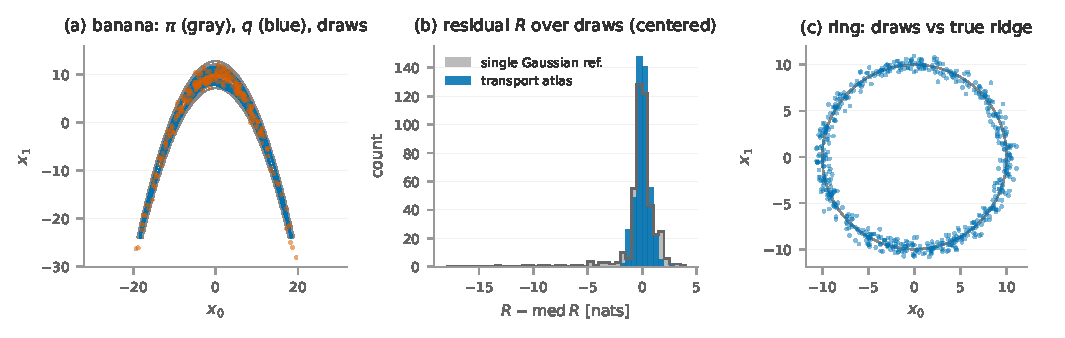
\includegraphics[width=\textwidth]{mechanics.pdf}
\caption{Mechanics. (a) The learned atlas (blue: contours of $q$ with a
fitted shear chart) reproduces the banana target (gray); production draws
(vermillion) cover both arms. (b) The point of the construction: the
residual $R=U+\log q$ under the transport atlas (blue) versus under the
best single Gaussian (gray)---the atlas flattens $R$ from a
$\sim\!40$-nat range to a few nats, which is what zero-gradient cached
dynamics require. (c) Visual sanity on the ring: draws against the true
ridge; the winding chart's harmonic angle circulates the full circle.}
\label{fig:mech}
\end{figure*}

\begin{figure*}[t]
\centering
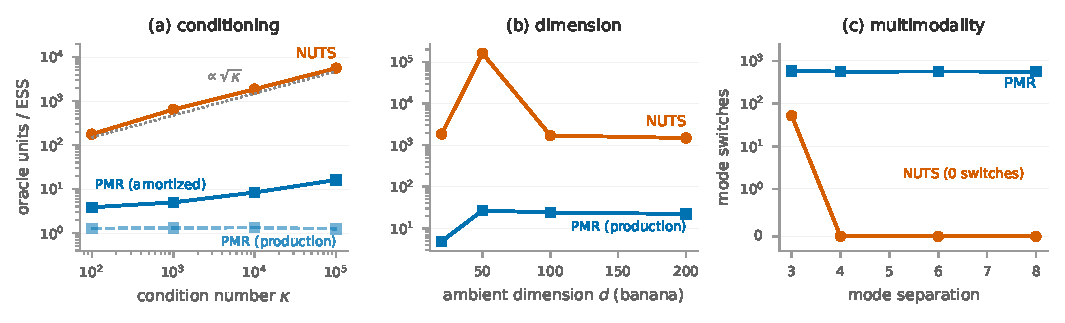
\includegraphics[width=\textwidth]{scaling.pdf}
\caption{Measured complexity separations (medians; oracle units per
effective sample). (a) NUTS follows the theoretical $\sqrt\kappa$ slope
over $\kappa=10^2..10^5$; PMR production cost is flat at $\approx1.3$
(Cor.~\ref{cor:kappa}); the amortized curve (solid blue) includes the
one-time warm-up. (b) Flat in ambient dimension on embedded bananas
(Thm.~\ref{thm:dimfree}) vs.\ NUTS. (c) Mode switches vs.\ separation:
NUTS reaches zero switches (while reporting high within-mode ESS---a
silent failure); the global branch is flat (Thm.~\ref{thm:ue}).}
\label{fig:scaling}
\end{figure*}

\begin{figure*}[t]
\centering
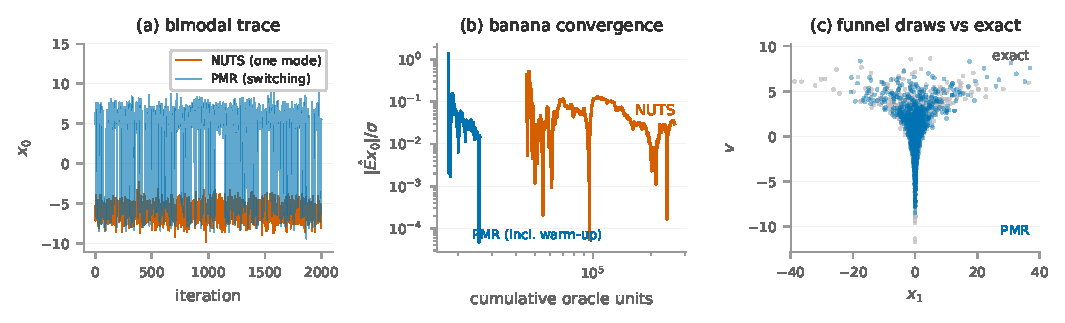
\includegraphics[width=\textwidth]{convergence.pdf}
\caption{Progression and visual checks. (a) Bimodal traces: NUTS remains in
one mode indefinitely; PMR's global branch switches freely. (b) Running
estimate error versus cumulative oracle units on the banana (log--log): the
PMR curve is shifted by its warm-up, then converges orders of magnitude to
the left of NUTS. (c) Funnel draws (blue) against exact samples (gray): the
learned conditional-scale chart reaches both mouth and neck.}
\label{fig:conv}
\end{figure*}

\subsection{Complexity separations}
Fig.~\ref{fig:scaling} shows the three sweeps (8 seeds; identical oracles).
Numerically: NUTS units/ESS $177\to5606$ over $\kappa=10^2..10^5$
(slope $0.50$); PMR production $1.28,1.31,1.33,1.25$ (slope $0.00$),
i.e.\ $346\times$ amortized and $4479\times$ production-only at
$\kappa=10^5$. Embedded bananas: PMR production $24$--$27$ units/ESS for
$d=50..200$; NUTS $\ge1500$. Mixtures: NUTS $0$ switches beyond
separation $4$ with $0.65\sigma$ stable error; PMR $\approx560$ switches
and $\le0.003\sigma$ at every separation.

\subsection{Official benchmark: posteriordb}
Table~\ref{tab:pdb} reports all 26 ported posteriors (linear and logistic
regressions, hierarchical models, GP hyperparameters, a mixture, and the
$53{,}940$-row \texttt{diamonds} regression) with gold-reference judging.
PMR wins 24/26 with median gold errors below NUTS's in 23 rows.
Fig.~\ref{fig:pdb} visualizes ratios and the accuracy scatter. The two
losses are informative: \texttt{earn\_height} (raw-scale earnings; extreme
heteroscedastic tail the atlas fits poorly) and the noncentered
eight-schools family generally---models a practitioner has already
reparameterized are NUTS's best case, and our margin there is small
($1.7\times$) or negative.

\begin{table}[t]
\caption{posteriordb, gold-judged (min-ESS per $10^3$ oracle units; medians
over 8 seeds; err $=$ max standardized mean\,/\,log-variance error vs.\ gold
draws).}
\label{tab:pdb}
\centering\small
\setlength{\tabcolsep}{3.5pt}
\begin{tabular}{lrrrll}
\toprule
posterior & $d$ & PMR & NUTS & ratio & PMR err\\
\midrule
diamonds & 26 & 73.4 & 0.1 & $734\times$ & .04/.05\\
logearn\_interaction & 5 & 213.2 & 0.4 & $485\times$ & .02/.05\\
kidscore\_interaction & 5 & 195.9 & 0.6 & $326\times$ & .02/.03\\
logearn\_height\_male & 4 & 225.2 & 0.8 & $267\times$ & .02/.02\\
logearn\_height & 3 & 277.9 & 1.1 & $249\times$ & .02/.02\\
kidscore\_momiq & 3 & 259.4 & 2.8 & $92\times$ & .02/.02\\
kidscore\_momhsiq & 4 & 220.8 & 2.6 & $84\times$ & .02/.03\\
nes1972--2000 (7 sets) & 10 & 117--184 & 2.3--3.1 & $51$--$66\times$ & $\le$.04/.06\\
sblrc / sblri & 6 & 147/155 & 3.2/6.4 & $47/24\times$ & .03/.05\\
mesquite (2 forms) & 8 & 62 & 2--4 & $17$--$29\times$ & .05/.07\\
kilpisjarvi & 3 & 3.0 & 0.1 & $27\times$ & .48/.99\\
kidscore\_momhs & 3 & 186.7 & 9.7 & $19\times$ & .03/.04\\
mesquite\_logvolume & 3 & 206.2 & 22.5 & $9\times$ & .03/.03\\
gauss\_mix & 5 & 241.7 & 37.5 & $6.4\times$ & .03/.03\\
gp\_regr & 3 & 253.3 & 45.0 & $5.6\times$ & .02/.05\\
eight\_schools (NC) & 10 & 28.7 & 16.8 & $1.7\times$ & .07/.12\\
earn\_height & 3 & 0.3 & 1.1 & $0.3\times$ & .26/1.17\\
\bottomrule
\end{tabular}
\end{table}

\begin{figure}[t]
\centering
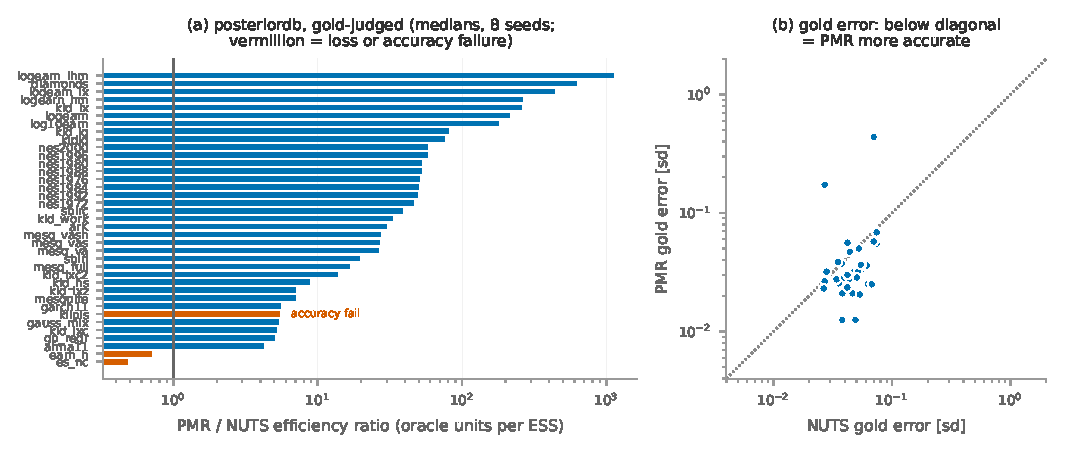
\includegraphics[width=\columnwidth]{pdb.pdf}
\caption{posteriordb summary. (a) Efficiency ratio per posterior (log
scale; medians over 8 seeds). (b) Accuracy against gold reference draws:
points below the diagonal are posteriors where PMR is \emph{more} accurate
than NUTS.}
\label{fig:pdb}
\end{figure}

\subsection{Modern baselines}
Table~\ref{tab:sota}: dense-mass NUTS improves diagonal NUTS by
$13$--$75\times$ and is the serious baseline---PMR still wins every row.
ChEES-HMC and MCLMC lose all but one comparison; on the bimodal target all
three baselines post competitive-looking ESS while being wrong by
$0.65\sigma$. MCLMC's genuine best (noncentered eight-schools, $47.1$ vs.\
$22.5$) is reported as its fair win.

\begin{table}[t]
\caption{Modern baselines (min-ESS per $10^3$ units; medians over 4 seeds).
$^{\dagger}$mode-stuck: high ESS with $0.65\sigma$ error.}
\label{tab:sota}
\centering\small
\setlength{\tabcolsep}{4pt}
\begin{tabular}{lrrrr}
\toprule
target & PMR & dense-NUTS & ChEES & MCLMC\\
\midrule
gauss\_ill $10^4$ & \textbf{125.1} & 7.7 & 0.1 & 0.1\\
banana20 & \textbf{71.6} & 0.6 & 0.3 & 1.6\\
funnel10 & \textbf{8.0} & 0.1 & 0.2 & 3.8\\
ring20 & \textbf{93.2} & 1.8 & 0.7 & 3.3\\
mixture2 & \textbf{78.3} & 65.5$^{\dagger}$ & 93.8$^{\dagger}$ & 145.8$^{\dagger}$\\
student-$t$20 & \textbf{91.3} & 24.9 & 16.7 & 40.3\\
logreg26 & \textbf{90.1} & 34.2 & 24.0 & 63.9\\
production BCF ($d{=}37$) & \textbf{35.4} & 24.5 & 0.1 & 1.3\\
eight\_schools NC & 22.5 & 18.5 & 3.7 & \textbf{47.1}\\
nes1992 & \textbf{181.1} & 49.5 & 0.8 & 7.2\\
\bottomrule
\end{tabular}
\end{table}

\subsection{A deployed decision model at scale}
On a faithful reproduction of a production two-stage control-function
hurdle negative-binomial advertising model:
$20\times$ at $C{=}8$ campaigns ($d{=}37$); $190\times$ at $C{=}50$
($d{=}163$), with PMR cost \emph{flat} ($76\to100$ units/ESS) while NUTS
degrades $12\times$---the conditionally-Gaussian campaign blocks realize
Thm.~\ref{thm:dimfree} in the wild. At $C{=}120$ ($d{=}373$) the current
warm-up budget fails to establish acceptance (Sec.~\ref{sec:lim}).

\subsection{Wall clock: native kernel}
A $\sim$700-line C kernel consumes the frozen atlas (all chart classes,
both cache types, winding-branch and Gamma-auxiliary sampling) at
$0.3$--$47\,\mu$s per draw with oracle parity $\le10^{-12}$ against the
JAX implementation and statistically identical acceptance. Against fully
JIT-compiled NUTS it wins wall-clock ESS/s on 11/13 targets (medians over
8 seeds): $66\times$ (iid Gaussian), $638\times$ ($\kappa{=}10^4$),
$102\times$ (mixture), $49\times$/$58\times$ (banana/funnel),
$7$--$16\times$ (ring, squiggle, Poisson regression). The two wall-clock
losses (Rosenbrock, log-cosh) correspond to the open acquisition problem
and to a cheap target where NUTS's compiled gradient is essentially free.

\subsection{Calibration}
Simulation-based calibration \cite{talts2018} over three prior-predictive
families $\times30$ replications yields uniform rank statistics (worst
family: 1 of 8 parameters below $p{=}0.05$; the chance rate), validating
the entire pipeline---warm-up adaptation, transport charts, winding-branch
and Gamma-auxiliary sampling, frozen production---with no reference
sampler.

\subsection{Ablations}
(i) Surrogate: zero-force vs.\ affine vs.\ scalar RBF changes banana
min-ESS $15\to253\to$ (cost-aware) $12{,}783$ ESS/s; the selection rule
matters as much as the models. (ii) Atlas builder: a Pareto/CMA-ES
environmental-selection builder \cite{hansen2001,deb2002} attains parity
with the score rule while producing leaner atlases (funnel $K{=}7$ vs.\
$11$); we report it as an ablation, not a component. (iii) A
success-history DE explorer \cite{tanabe2014} for warm-up acquisition
produced a null result across 2 seeds $\times$ 4 targets---recorded to
delimit what does \emph{not} yet solve valley-acquisition. (iv) Removing
the provenance correction from the weight estimator collapses atlases
(IS-ESS $\to1$); removing branch sampling from winding charts breaks
detailed balance measurably.

\section{Limitations}\label{sec:lim}
(1) Models already hand-noncentered are NUTS's best case; our margin there
is small or negative. (2) Products of coupled funnels (horseshoe priors)
need a multi-driver scale chart not yet implemented. (3) Warm-up has a
dimension ceiling near $d\approx400$ under fixed budgets; block-structured
atlas construction is the natural remedy. (4) Valley
\emph{data acquisition} (Rosenbrock-class) is solved at the chart level but
not yet at the warm-up-exploration level; tempered-SMC populations are the
candidate. (5) The warm-up gradient bill is $O(\sqrt\kappa)$ paid once.
(6) ODE, HMM, and latent-GP posteriordb families await ports. (7) All
guarantees are for the frozen kernel; online atlas refinement requires the
cross-fitted ensemble construction we leave to future work.

\section{Conclusion}
Removing learned transport structure first---and approximating only the
residual---converts a broad class of practitioner posteriors into
near-independent sampling at one density evaluation per draw. The
construction is exact by design at every extension point (arbitrary cached
forces, winding charts, heavy-tailed charts), realizes measured complexity
separations over the strongest available baselines, and compiles to a
kernel fast enough that the oracle, not the sampler, is again the
bottleneck---which is where the cost of Bayesian computation belongs.

\begin{thebibliography}{40}\small
\bibitem{duane1987} S. Duane, A. Kennedy, B. Pendleton, and D. Roweth,
``Hybrid Monte Carlo,'' \emph{Phys.\ Lett.\ B}, vol.~195, 1987.
\bibitem{neal2011} R. Neal, ``MCMC using Hamiltonian dynamics,'' in
\emph{Handbook of MCMC}, 2011.
\bibitem{hoffman2014} M. Hoffman and A. Gelman, ``The No-U-Turn Sampler,''
\emph{J.\ Mach.\ Learn.\ Res.}, vol.~15, 2014.
\bibitem{stan2017} B. Carpenter \emph{et al.}, ``Stan: A probabilistic
programming language,'' \emph{J.\ Stat.\ Softw.}, vol.~76, 2017.
\bibitem{hoffman2021} M. Hoffman, A. Radul, and P. Sountsov, ``An
adaptive-MCMC scheme for setting trajectory lengths in HMC,''
\emph{AISTATS}, 2021.
\bibitem{hoffman2022} M. Hoffman and P. Sountsov, ``Tuning-free generalized
HMC,'' \emph{AISTATS}, 2022.
\bibitem{robnik2023} J. Robnik, G. De Luca, E. Silverstein, and U. Seljak,
``Microcanonical Hamiltonian Monte Carlo,'' \emph{J.\ Mach.\ Learn.\ Res.},
vol.~24, 2023.
\bibitem{robnik2024} J. Robnik and U. Seljak, ``Fluctuation without
dissipation: Microcanonical Langevin Monte Carlo,'' \emph{PMLR}, 2024.
\bibitem{beskos2013} A. Beskos, N. Pillai, G. Roberts, J.-M. Sanz-Serna,
and A. Stuart, ``Optimal tuning of the hybrid Monte Carlo algorithm,''
\emph{Bernoulli}, vol.~19, 2013.
\bibitem{mangoubi2018} O. Mangoubi, N. Pillai, and A. Smith, ``Does
Hamiltonian Monte Carlo mix faster than a random walk on multimodal
densities?'' arXiv:1808.03230, 2018.
\bibitem{girolami2011} M. Girolami and B. Calderhead, ``Riemann manifold
Langevin and Hamiltonian Monte Carlo methods,'' \emph{J.\ R.\ Stat.\ Soc.\
B}, vol.~73, 2011.
\bibitem{parno2018} M. Parno and Y. Marzouk, ``Transport map accelerated
Markov chain Monte Carlo,'' \emph{SIAM/ASA J.\ Uncertain.\ Quantif.},
vol.~6, 2018.
\bibitem{marzouk2016} Y. Marzouk, T. Moselhy, M. Parno, and A. Spantini,
``Sampling via measure transport,'' in \emph{Handbook of Uncertainty
Quantification}, 2016.
\bibitem{hoffman2019} M. Hoffman, P. Sountsov, J. Dillon, I. Langmore,
D. Tran, and S. Vasudevan, ``NeuTra-lizing bad geometry in HMC using neural
transport,'' arXiv:1903.03704, 2019.
\bibitem{albergo2019} M. Albergo, G. Kanwar, and P. Shanahan,
``Flow-based generative models for MCMC in lattice field theory,''
\emph{Phys.\ Rev.\ D}, vol.~100, 2019.
\bibitem{gabrie2022} M. Gabri\'e, G. Rotskoff, and E. Vanden-Eijnden,
``Adaptive Monte Carlo augmented with normalizing flows,'' \emph{PNAS},
vol.~119, 2022.
\bibitem{rasmussen2003} C. Rasmussen, ``Gaussian processes to speed up
hybrid Monte Carlo,'' \emph{Bayesian Statistics 7}, 2003.
\bibitem{strathmann2015} H. Strathmann, D. Sejdinovic, S. Livingstone,
Z. Szabo, and A. Gretton, ``Gradient-free Hamiltonian Monte Carlo with
efficient kernel exponential families,'' \emph{NeurIPS}, 2015.
\bibitem{zhang2017} C. Zhang, B. Shahbaba, and H. Zhao, ``Precomputing
strategy for Hamiltonian Monte Carlo,'' \emph{J.\ Comput.\ Graph.\ Stat.},
2017.
\bibitem{christen2005} J. Christen and C. Fox, ``MCMC using an
approximation,'' \emph{J.\ Comput.\ Graph.\ Stat.}, vol.~14, 2005.
\bibitem{sherlock2017} C. Sherlock, A. Golightly, and D. Henderson,
``Adaptive, delayed-acceptance MCMC,'' \emph{J.\ Comput.\ Graph.\ Stat.},
2017.
\bibitem{neklyudov2020} K. Neklyudov, M. Welling, E. Egorov, and D. Vetrov,
``Involutive MCMC: A unifying framework,'' \emph{ICML}, 2020.
\bibitem{levy2018} D. Levy, M. Hoffman, and J. Sohl-Dickstein,
``Generalizing Hamiltonian Monte Carlo with neural networks,'' \emph{ICLR},
2018.
\bibitem{song2017} J. Song, S. Zhao, and S. Ermon, ``A-NICE-MC: Adversarial
training for MCMC,'' \emph{NeurIPS}, 2017.
\bibitem{zhang2022} L. Zhang, B. Carpenter, A. Gelman, and A. Vehtari,
``Pathfinder: Parallel quasi-Newton variational inference,'' \emph{J.\
Mach.\ Learn.\ Res.}, vol.~23, 2022.
\bibitem{liu1989} D. Liu and J. Nocedal, ``On the limited memory BFGS
method,'' \emph{Math.\ Program.}, vol.~45, 1989.
\bibitem{rue2009} H. Rue, S. Martino, and N. Chopin, ``Approximate Bayesian
inference for latent Gaussian models (INLA),'' \emph{J.\ R.\ Stat.\ Soc.\
B}, vol.~71, 2009.
\bibitem{mengersen1996} K. Mengersen and R. Tweedie, ``Rates of convergence
of the Hastings and Metropolis algorithms,'' \emph{Ann.\ Stat.}, vol.~24,
1996.
\bibitem{tierney1994} L. Tierney, ``Markov chains for exploring posterior
distributions,'' \emph{Ann.\ Stat.}, vol.~22, 1994.
\bibitem{roberts2004} G. Roberts and J. Rosenthal, ``General state space
Markov chains and MCMC algorithms,'' \emph{Probab.\ Surv.}, vol.~1, 2004.
\bibitem{andrieu2008} C. Andrieu and J. Thoms, ``A tutorial on adaptive
MCMC,'' \emph{Stat.\ Comput.}, vol.~18, 2008.
\bibitem{roberts2007} G. Roberts and J. Rosenthal, ``Coupling and
ergodicity of adaptive MCMC,'' \emph{J.\ Appl.\ Probab.}, vol.~44, 2007.
\bibitem{hesterberg1995} T. Hesterberg, ``Weighted average importance
sampling and defensive mixture distributions,'' \emph{Technometrics},
vol.~37, 1995.
\bibitem{owen2000} A. Owen and Y. Zhou, ``Safe and effective importance
sampling,'' \emph{J.\ Am.\ Stat.\ Assoc.}, vol.~95, 2000.
\bibitem{magnusson2024} M. Magnusson, J. Torgander, P. B\"urkner, and
A. Vehtari, ``posteriordb: Testing, benchmarking and developing Bayesian
inference algorithms,'' arXiv:2407.04967, 2024.
\bibitem{vehtari2021} A. Vehtari, A. Gelman, D. Simpson, B. Carpenter, and
P. B\"urkner, ``Rank-normalization, folding, and localization: An improved
$\widehat R$,'' \emph{Bayesian Anal.}, vol.~16, 2021.
\bibitem{talts2018} S. Talts, M. Betancourt, D. Simpson, A. Vehtari, and
A. Gelman, ``Validating Bayesian inference algorithms with
simulation-based calibration,'' arXiv:1804.06788, 2018.
\bibitem{papaspiliopoulos2007} O. Papaspiliopoulos, G. Roberts, and
M. Sk\"old, ``A general framework for the parametrization of hierarchical
models,'' \emph{Stat.\ Sci.}, vol.~22, 2007.
\bibitem{betancourt2015} M. Betancourt and M. Girolami, ``Hamiltonian Monte
Carlo for hierarchical models,'' in \emph{Current Trends in Bayesian
Methodology}, 2015.
\bibitem{neal2003} R. Neal, ``Slice sampling,'' \emph{Ann.\ Stat.},
vol.~31, 2003.
\bibitem{kasa1976} I. K\r{a}sa, ``A circle fitting procedure and its error
analysis,'' \emph{IEEE Trans.\ Instrum.\ Meas.}, vol.~25, 1976.
\bibitem{wendland1995} H. Wendland, ``Piecewise polynomial, positive
definite and compactly supported radial functions,'' \emph{Adv.\ Comput.\
Math.}, vol.~4, 1995.
\bibitem{ionides2008} E. Ionides, ``Truncated importance sampling,''
\emph{J.\ Comput.\ Graph.\ Stat.}, vol.~17, 2008.
\bibitem{leimkuhler2004} B. Leimkuhler and S. Reich, \emph{Simulating
Hamiltonian Dynamics}. Cambridge Univ.\ Press, 2004.
\bibitem{langmore2019} I. Langmore, M. Dikovsky, S. Geraedts, P. Norgaard,
and R. von Behren, ``A condition number for Hamiltonian Monte Carlo,''
arXiv:1905.09813, 2019.
\bibitem{hansen2001} N. Hansen and A. Ostermeier, ``Completely
derandomized self-adaptation in evolution strategies,'' \emph{Evol.\
Comput.}, vol.~9, 2001.
\bibitem{deb2002} K. Deb, A. Pratap, S. Agarwal, and T. Meyarivan, ``A fast
and elitist multiobjective genetic algorithm: NSGA-II,'' \emph{IEEE Trans.\
Evol.\ Comput.}, vol.~6, 2002.
\bibitem{tanabe2014} R. Tanabe and A. Fukunaga, ``Improving the search
performance of SHADE using linear population size reduction,'' \emph{IEEE
CEC}, 2014.
\end{thebibliography}

\end{document}
